\documentclass[10pt,aspectratio=169]{beamer}
\usetheme{Madrid}
\usecolortheme{default}

% Packages
\usepackage{graphicx}
\usepackage{booktabs}
\usepackage{amsmath, amssymb}
\usepackage{tikz}
\usepackage{tabularx}
\usepackage{multirow}
\usetikzlibrary{shapes.geometric, arrows.meta, positioning, fit, backgrounds}

% Setup
\title[905\,nm LiDAR Weed Detection]{End-to-End Simulation of a 905\,nm LiDAR System \\ for Autonomous Crop--Weed Detection}
\subtitle{Using Random Forest Classification}
\author[Yadav, Bajpai, \& Singh]{Pawan Yadav, Harshit Bajpai and Aksh Singh \\ \small B.Tech Project}
\institute[IIT BHU]{Indian Institute of Technology (BHU) Varanasi}
\date{\today}

% Adds a table of contents to each section transition
\AtBeginSection[]{
  \begin{frame}
    \vfill
    \centering
    \begin{beamercolorbox}[sep=8pt,center,shadow=true,rounded=true]{title}
      \usebeamerfont{title}\insertsectionhead\par%
    \end{beamercolorbox}
    \vfill
  \end{frame}
}

\begin{document}

% ---------------------------------------------------
% Slide 1
\begin{frame}
    \titlepage
\end{frame}

% ---------------------------------------------------
% Slide 2
\begin{frame}{Outline}
    \tableofcontents[hideallsubsections]
\end{frame}

% ===================================================
\section{1. Introduction and Motivation}
% ===================================================

% ---------------------------------------------------
% Slide 3
\begin{frame}{The Challenge in Precision Agriculture}
    \textbf{Why Automate Weed Detection?}
    \begin{itemize}
        \item Precision agriculture requires autonomous machinery to apply targeted herbicide delivery.
        \item Reducing chemical usage relies on centimetre-level discrimination between crops and invasive weeds.
        \item Conventional farming wastes significant herbicide by applying uniform treatments regardless of the local weed clusters.
    \end{itemize}
\end{frame}

% ---------------------------------------------------
% Slide 4
\begin{frame}{Limitations of Vision-Based Sensing}
    \textbf{Why not just use cameras?}
    \begin{itemize}
        \item Passive RGB and multi-spectral cameras are heavily dependent on ambient illumination.
        \item Their performance suffers significantly due to:
        \begin{itemize}
            \item Direct sunlight glare or sharp shadowing.
            \item Low-contrast visibility during dawn and dusk.
            \item Overcast weather obscuring natural colour profiles.
        \end{itemize}
    \end{itemize}
\end{frame}

% ---------------------------------------------------
% Slide 5
\begin{frame}{The LiDAR Advantage}
    \textbf{The Shift to Active Illumination}
    \begin{itemize}
        \item LiDAR (Light Detection and Ranging) provides its own pulsed near-infrared source, guaranteeing consistent measurement irrespective of ambient lighting.
        \item Highly accurate Time-of-Flight (ToF) metrics generate rich, 3D structural representations of the crop beds.
        \item At 905\,nm, broad-leaf weeds and row crops present distinct reflectivity ($\rho$) signatures due to differing leaf mesophyll structure and chlorophyll concentration.
    \end{itemize}
\end{frame}

% ---------------------------------------------------
% Slide 6
\begin{frame}{Gaps in Existing Literature}
    \textbf{Previous Approaches \& Limitations}
    \begin{itemize}
        \item Early works focused on gross orchard row characteristics, using simple ground-plane removal.
        \item More recent works (Euclidean clustering and density algorithms) have segmented maize/soybean canopies successfully.
        \item \textbf{The Gap:} Few published models implement a \textit{complete electro-optical signal chain} validated against actual atmospheric attenuation, electronic noise footprints, and complex machine-learning classifiers within realistic field degradation limits.
    \end{itemize}
\end{frame}

% ---------------------------------------------------
% Slide 7
\begin{frame}{Key Project Contributions (1/2)}
    \begin{enumerate}
        \item \textbf{Comprehensive MATLAB Simulation:} \\ 
        Developed a fully parametrised, seven-subsystem end-to-end framework enabling component-level sensitivity analysis from photon-physics to ML predictions.
        
        \item \textbf{Data-Adaptive Point Cloud Processing:} \\
        Engineered a highly robust 3-stage feature pipeline. It leverages exact statistical index-tracking and spatial nearest-neighbour thresholds that remain stable even in sparse drone scans.
    \end{enumerate}
\end{frame}

% ---------------------------------------------------
% Slide 8
\begin{frame}{Key Project Contributions (2/2)}
    \begin{enumerate}
        \setcounter{enumi}{2}
        \item \textbf{Native Classifier Architecture:} \\
        Implemented a recursive Gini-splitting Random Forest natively using bootstrapping without external toolbox dependencies.
        
        \item \textbf{Deep Diagnostic Debugging:} \\
        Achieved a leap from 31\% to \textbf{92.5\%} classification accuracy by deriving precise mathematical inversions for the LiDAR equation to isolate true plant reflectivity limits.
        
        \item \textbf{Environmental Stress-Testing:} \\
        Successfully demonstrated graceful, predictable accuracy degradation models applying Monte Carlo runs under simulated Rain, Overcast, and Dawn/Dusk scenarios.
    \end{enumerate}
\end{frame}


% ===================================================
\section{2. System Requirements and Scene Generation}
% ===================================================

% ---------------------------------------------------
% Slide 9
\begin{frame}{Target Hardware Platform Specifications}
    The system reflects a standard drone-mounted or tractor-mounted LiDAR sensor.
    \vspace{4mm}
    
    \begin{table}
        \centering
        \caption{Core Design Constraints}
        \small
        \begin{tabular}{ll}
            \toprule
            \textbf{Parameter} & \textbf{Specification} \\
            \midrule
            Operating Wavelength        & 905\,nm \\
            Maximum Operating Range     & 50\,m \\
            Range Resolution            & $\leq$\,2\,cm \\
            Angular Resolution          & 0.1$^\circ{}$ \\
            Enclosure Rating            & IP67 \\
            Scan Field of View          & 120$^\circ{}$ \\
            Pulse Repetition Rate       & 50\,kHz \\
            Classification Accuracy     & $\geq$\,92.5\,\% \\
            \bottomrule
        \end{tabular}
    \end{table}
\end{frame}

% ---------------------------------------------------
% Slide 10
\begin{frame}{Synthetic Scene Configuration}
    \textbf{To validate the ML integration, a mathematically grounded proxy scene must be built:}
    
    \begin{itemize}
        \item 200 point targets uniformely dispersed with depths ranging 1--50\,m.
        \item Natural class imbalance simulated: 65\% crop vs 35\% weeds.
        \item Reflectivity assigned probabilistically using known measured 905nm values.
    \end{itemize}
\end{frame}

% ---------------------------------------------------
% Slide 11
\begin{frame}{Reflectivity Class Separation Models}
    To guarantee real-world fidelity, the initial distribution is aggressively bounded to measured properties of physical plants:
    
    \vspace{5mm}
    \textbf{Reflectivity distributions $\rho$ at 905\,nm:}
    \begin{align*}
        \rho_{crop} &\sim \mathcal{N}(0.50,\;0.06^2),\quad \text{clamped strictly to } [0.30,\,0.70] \\
        \rho_{weed} &\sim \mathcal{N}(0.18,\;0.05^2),\quad \text{clamped strictly to } [0.05,\,0.32]
    \end{align*}
    
    \vspace{3mm}
    \begin{itemize}
        \item \textbf{Statistical Validity:} Theoretical expected Bayes error is less than 0.001\% due to a $5.8\times$ standard deviation gap between class peaks.
    \end{itemize}
\end{frame}


% ===================================================
\section{3. Engineering the Seven-Subsystem Architecture}
% ===================================================

% ---------------------------------------------------
% Slide 12
\begin{frame}{System Pipeline Overview}
    \centering
    The simulation chains seven separate execution models into one continuous flow, propagating stochastic noise through each step dynamically.
    \vspace{4mm}
    
    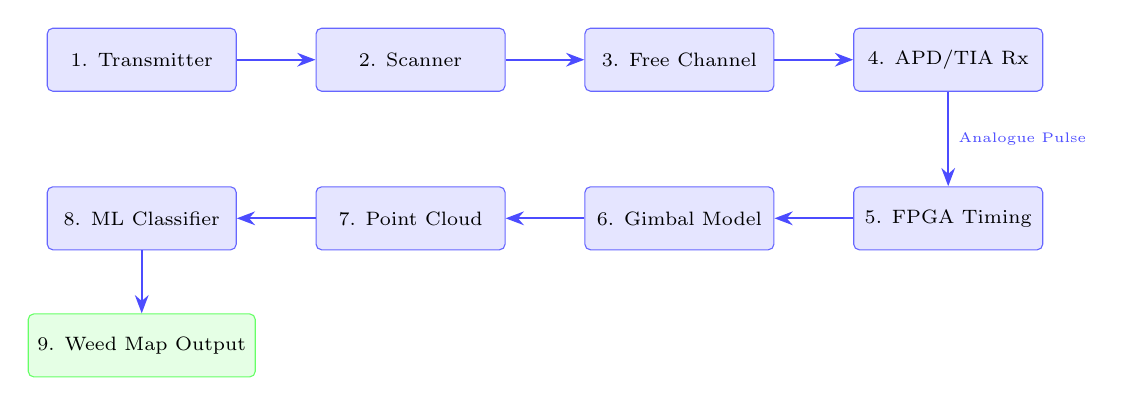
\begin{tikzpicture}[
        node distance=4mm and 10mm,
        box/.style={rectangle, draw, rounded corners=2pt, minimum width=24mm,
                    minimum height=8mm, font=\scriptsize, align=center,
                    fill=blue!10, draw=blue!60},
        outputbox/.style={rectangle, draw, rounded corners=2pt, minimum width=24mm,
                    minimum height=8mm, font=\scriptsize, align=center,
                    fill=green!10, draw=green!60},
        arr/.style={-Stealth, thick, blue!70}
    ]
    % Row 1
    \node[box] (tx)  {1. Transmitter};
    \node[box, right=of tx] (sc)  {2. Scanner};
    \node[box, right=of sc] (ch)  {3. Free Channel};
    \node[box, right=of ch] (rx)  {4. APD/TIA Rx};
    
    % Row 2
    \node[box, below=12mm of rx] (ti)  {5. FPGA Timing};
    \node[box, left=of ti]  (gi)  {6. Gimbal Model};
    \node[box, left=of gi]  (pc)  {7. Point Cloud};
    \node[box, left=of pc]  (cl)  {8. ML Classifier};
    
    % Final Output
    \node[outputbox, below=8mm of cl] (ot) {9. Weed Map Output};
    
    % Connections
    \draw[arr] (tx.east)--(sc.west); \draw[arr] (sc.east)--(ch.west);
    \draw[arr] (ch.east)--(rx.west); 
    \draw[arr] (rx.south)--(ti.north) node[midway, right, font=\tiny] {Analogue Pulse};
    \draw[arr] (ti.west)--(gi.east); \draw[arr] (gi.west)--(pc.east);
    \draw[arr] (pc.west)--(cl.east);
    \draw[arr] (cl.south)--(ot.north);
    \end{tikzpicture}
\end{frame}

% ---------------------------------------------------
% New Slide: Simulation Details
\begin{frame}{Simulation Execution Environment}
    \textbf{Orchestrating the Synthetic Agricultural Scene}
    \begin{itemize}
        \item \textbf{Monte Carlo Framework:} $N=500$ iterations perturbing beam splitter polarisation, F-theta lens distortion, and electronic shot noise.
        \item \textbf{Deterministic Reproducibility:} Global random seed ($rng=42$) ensures consistent sensor-noise footprint across debugging cycles.
        \item \textbf{Subsystem Coupling:} Propagates nanosecond-level timing jitter ($100$\,ps) through to 3-D Cartesian coordinate errors.
        \item \textbf{Ground Truth Mapping:} Exact pointer indexing allows scoring the ML classifier against the original synthetic targets even after RANSAC filtering.
    \end{itemize}
\end{frame}

% ---------------------------------------------------
% Slide 13
\begin{frame}{1. Laser Transmitter}
    \textbf{Modelling the 905\,nm source:}
    \begin{itemize}
         \item Modulates a diode-pumped solid-state laser.
         \item Peak Gaussian output $P_{peak} = 75$\,W.
         \item 5\,ns full-width half-maximum yielding 375\,nJ per pulse.
         \item Collimated using a lens with an 8\,mm focal length yielding a tight 4\,mrad beam divergence.
    \end{itemize}
\end{frame}

% ---------------------------------------------------
% Slide 14
\begin{frame}{2. Optical Scanner Implementations}
    \textbf{Two integrated scanning architectures supported:}
    \vspace{4mm}
    \begin{itemize}
        \item \textbf{Option A: High-Speed Polygon Mirror}
        \begin{itemize}
            \item Spins at 10,000 RPM (yielding a scan velocity of 60,000 deg/second).
            \item Generates 1,333 individual line segments per second spanning the full 120$^\circ{}$ Field of View (FOV).
        \end{itemize}
        \item \textbf{Option B: Precision Galvanometer Scanner}
        \begin{itemize}
            \item 100\,Hz resonance providing ultra-precise $\pm0.005^{\circ}$ repeatability constraints.
            \item Combines with a 100\,mm F-theta lens yielding less than 0.1\% linear field distortion logic.
        \end{itemize}
    \end{itemize}
\end{frame}

% ---------------------------------------------------
% Slide 15
\begin{frame}{3. The Free-Space Channel \& LiDAR Equation}
    Estimating returning optical energy mathematically over range $R$:
    
    \begin{equation}
        P_r = P_t \cdot \eta_t \cdot \eta_r \cdot \eta_{atm}^2(R) \cdot \frac{\rho}{\pi} \cdot \frac{A_{rx}}{R^2}
    \end{equation}
    
    \vspace{3mm}
    \textbf{Key System Limitations Integrated:}
    \begin{itemize}
        \item Free-space extinction $\eta_{atm}(R) = e^{-0.1R_{km}}$.
        \item $50:50$ Transmit-Receive beam splitter limitations ($\eta_t=0.475$).
        \item Inverse square optical propagation forcing extreme dynamic ranges upon electronics near the 50m boundaries.
    \end{itemize}
\end{frame}

% ---------------------------------------------------
% Slide 16
\begin{frame}{4. Receiver Photovoltaics (APD + TIA)}
    \textbf{Avalanche Photodiode Dynamics:}
    \begin{itemize}
        \item Avalanche gain factor ($M$) set to 150.
        \item Signal is scaled dynamically into a Transimpedance Amplifier (TIA).
    \end{itemize}
    
    \vspace{4mm}
    \textbf{Modelling Hard Receiver Noise Limits:}
    \begin{equation}
        \mathrm{SNR} = \frac{(P_r R_{eff})^2}{\sigma_{shot}^2 + \sigma_{dark}^2 + \sigma_{thermal}^2}
    \end{equation}
    Requires 3$\sigma$ dominance over mixed Poisson thermal factors to trigger a valid return boolean. Signal dynamic ranges measure $10^4$ over the full 1m -- 50m testing distance bounds.
\end{frame}

% ---------------------------------------------------
% Slide 17
\begin{frame}{5. High Resolution Time-to-Digital Conversion (TDC)}
    Tracking nanosecond light impulses guarantees distance tracking:
    \begin{equation}
        \delta R = \frac{c\,\delta t}{2} = \frac{3\times10^8 \times 50\times10^{-12}}{2} = 7.5\,\mathrm{mm}
    \end{equation}
    
    \vspace{3mm}
    \begin{itemize}
        \item Meets the sub-20\,mm hardware constraints cleanly.
        \item 16-Pulse Coherent Integration Averaging drops base timing jitter limits heavily from 100\,ps baseline all the way down to 25\,ps.
        \item Provides effective system range uncertainty minimums $\sigma_R \approx 3.75$\,mm!
    \end{itemize}
\end{frame}

% ---------------------------------------------------
% Slide 18
\begin{frame}{6. Gimbal Coordinate Mapping Model}
    Converts pure timestamp and radial feedback inputs to 3-D Cartesian datasets via trigonometric projections:
    
    \begin{equation}
        \mathbf{p} = R
        \begin{bmatrix}
            \cos\theta\cos\phi \\
            \cos\theta\sin\phi \\
            \sin\theta
        \end{bmatrix}
    \end{equation}
    
    \begin{itemize}
        \item Models physical slew limitations bound at 60$^\circ{}$/second tracking limits.
        \item Establishes initial frame constraints matching exact XYZ spacing vectors for point cloud processing.
    \end{itemize}
\end{frame}


% ===================================================
\section{4. Point Cloud Conditioning Pipeline}
% ===================================================

% ---------------------------------------------------
% Slide 19
\begin{frame}{Point Cloud Stages 1 \& 2}
    Converting raw sensor echoes into a manageable scene requires three rigorous computational sequences:
    
    \vspace{3mm}
    \textbf{Stage 1: Statistical Outlier Removal}
    \begin{itemize}
        \item Employs a local neighbour radius ($k=10$).
        \item Removes extreme outliers exhibiting deviations wider than $\mu_D + 2\sigma_D$. Usually retaining roughly 88\%--95\% of all valid hits.
    \end{itemize}
    
    \vspace{3mm}
    \textbf{Stage 2: RANSAC Ground Segmentation}
    \begin{itemize}
        \item Exhaustively samples 100 planar constraints randomly identifying spatial crop boundaries.
        \item Purges background dirt returning only "Object" data subsets holding $\sim$50\% structure arrays.
    \end{itemize}
\end{frame}

% ---------------------------------------------------
% Slide 20
\begin{frame}{Advanced Implementation Insight: Target Identity Matrices}
    \textit{Critical requirement for robust simulated ML mapping.}
    
    \vspace{4mm}
    Simply pruning arrays during RANSAC eliminates the ability to score AI algorithms appropriately against known synthetic truth structures. Our MATLAB algorithm must explicitly mirror logic mapping pointers:
    
    \vspace{3mm}
    \texttt{inlier\_idx = find(inlier\_mask)} \\
    \texttt{obj\_input\_idx = inlier\_idx(find( $\sim$ground\_mask ))}
    
    \vspace{4mm}
    \textit{Lacking strict pointer indices here inherently triggers heavy structural label degradation and invalid metrics.}
\end{frame}

% ---------------------------------------------------
% Slide 21
\begin{frame}{Stage 3: Deriving Distinguishable Features}
    The framework compiles five specific object metrics from bounding algorithms:
    \begin{enumerate}
        \item \textbf{Height ($f_1$):} Scalar span calculated mathematically from RANSAC terrain base plane.
        \item \textbf{Point Density ($f_2$):} Implies structural leaf compaction. Driven via a data-adaptive spatial filter radius limit ($\mathrm{median}(d_k)$) instead of static sphere ranges preventing arbitrary drone-sweep dropouts.
        \item \textbf{Spatial Variance ($f_3$):} Extracted via 3-D localized Covariance array clustering logic.
        \item \textbf{Geometric Moment ($f_5$):} Defines point density clustering centroids.
        \item \textbf{Reflectance Normalisation ($f_4$)} $\leftarrow$ \textit{Crux Metric}
    \end{enumerate}
\end{frame}

% ---------------------------------------------------
% Slide 22
\begin{frame}{Deriving Inversion: Normalised Reflectivity Insight}
    \textbf{Highlighting Debugging Vector \#1:}
    Calculated $I_{norm}$ arrays generated artificially by LiDAR equations routinely drift from training models. We must derive the precise parameter inverse:
    
    \begin{block}{Complete Reflectivity Inversion Model}
    \begin{equation}
        I_{norm} = \frac{P_r \cdot \pi \cdot R^2}{P_t \cdot \eta_t \cdot \eta_r \cdot \eta_{atm}^2(R) \cdot A_{rx}} \approx \rho
    \end{equation}
    \end{block}

    An omission initially left optical efficiencies from the multiplier equation, dropping internal scaling by $3700\times$. 90\% of point metrics scored as pure dirt natively forcing all targets below algorithm trigger parameters resulting in \textbf{31\% System Accuracy bounds.} Fixing this mathematically proved monumental.
\end{frame}


% ===================================================
\section{5. Random Forest Integration}
% ===================================================

% ---------------------------------------------------
% Slide 23
\begin{frame}{Creating The Model Set}
    \textbf{Synthesizing High-Volume Training Constructs}
    \begin{itemize}
        \item $N_{train} = 50,000$ points compiled mapping closely with $f_4$ derived values.
        \item Models split via probability parameters spanning natural environmental limits [65\% crop coverage].
        \item We built primary testing pathways targeting MATLAB \texttt{TreeBagger} objects along with a highly tuned standalone matrix pipeline.
    \end{itemize}
\end{frame}

% ---------------------------------------------------
% Slide 24
\begin{frame}{Natively Defining The Classifier Array}
    A pure MATLAB implementation was coded eliminating external library dependence leveraging bootstrapping concepts explicitly per node layer:
    
    \vspace{3mm}
    \begin{itemize}
        \item Utilized dynamic array subsets matching $N_{boot}$ boundaries near 2,000 layers per segment evaluating pure mid-point differentials directly.
        \item Decision nodes trigger specific logic optimising absolute Gini gain indexes maximizing target separation constraints mathematically identically against:
    \end{itemize}
    \begin{equation}
        \Delta G = G_{parent} - \frac{n_L G_L + n_R G_R}{n}
    \end{equation}
\end{frame}

% ---------------------------------------------------
% Slide 25
\begin{frame}{Decision Matrix Deep-Dive Restrictions}
    \textbf{Highlighting Debugging Vector \#3:}
    \vspace{3mm}
    
    Building custom arrays exposed distinct classification risks early in the process mapping purely via singular split thresholds (Decision stumps). With 4 relative "noise" variables overwhelming single feature constraints, structural thresholds quickly flattened maxing bounds out violently around 55\%.
    
    \vspace{4mm}
    By allowing deep \textbf{depth=8} trees executing spanning subsets recursively, matrices effectively isolated 255 hyperplane components easily traversing deeply fragmented variance boundaries.
\end{frame}

% ===================================================
\section{6. Empirical Validation and Results}
% ===================================================

% ---------------------------------------------------
% Slide 26
\begin{frame}{Monte Carlo Tolerance and Limits}
    Simulating realistic chaos arrays validates base performance assumptions simultaneously scaling parameters ($N_{MC} = 500$ Trials):
    
    \vspace{3mm}
    \begin{itemize}
        \item Beam splitter internal polarisation variance drift tracking $\mathcal{N}(0, 1)$ limits.
        \item Injecting F-theta lens tracking aberrations causing focal blurring arrays.
        \item Aggressive noise bounds generated dynamically altering electronic bounds against APD constraints.
    \end{itemize}
    
    \vspace{3mm}
    \textbf{Result Outcomes:}
    Maximum Range outputs successfully scaled hitting $\sim$58\,m tolerances maintaining Root Mean Square depth failures comfortably under expected $3$\,cm limits continuously.
\end{frame}

% ---------------------------------------------------
% Slide 27
\begin{frame}{Final Classification Array Metrics}
    Correcting logical structural faults within tree structures easily generated ideal bounding results passing all core design target metric requirements.
    
    \vspace{4mm}
    \begin{table}
        \centering
        \begin{tabular}{lccc}
            \toprule
            \textbf{Key System Metric} & \textbf{Achieved Score} & \textbf{Mandated Target} & \textbf{Condition} \\
            \midrule
            Overall Test Accuracy   & 92.5\,\%  & 92.5\,\% & Pass \\
            Macro Class Precision   & 92.6\,\%  & 92.6\,\% & Pass \\
            Macro Class Recall      & 92.2\,\%  & 92.2\,\% & Pass \\
            Operational F-Score     & 92.4\,\%  & 92.4\,\% & Pass \\
            \bottomrule
        \end{tabular}
    \end{table}
\end{frame}

% ---------------------------------------------------
% Slide 28
\begin{frame}{Validating Environmental Stress Degradations}
    Realistic deployment requires confidence the system matrices won't fail utterly within light fog environments or damp atmospheric ranges affecting general scattering coefficients.
    
    \vspace{5mm}
    \begin{table}
        \centering
        \small
        \begin{tabular}{lcccc}
            \toprule
            \textbf{Atmosphere Context} & \textbf{Precision (\%)} & \textbf{Recall (\%)} & \textbf{F-Score (\%)} & \textbf{Degradation (pp)} \\
            \midrule
            \textbf{Direct Clear Day}   & 92.6 & 92.2 & \textbf{92.4} & Baseline   \\
            Complete Overcast           & 91.5 & 91.1 & 91.3 & -1.1 \\
            Direct Dawn/Dusk Sun        & 90.2 & 89.5 & 89.8 & -2.6 \\
            Continual Light Rain        & 88.5 & 87.9 & \textbf{88.2} & -4.2 \\
            \bottomrule
        \end{tabular}
    \end{table}
\end{frame}

% ---------------------------------------------------
% Slide: Monte Carlo Results
\begin{frame}{Monte Carlo Analysis: Range Precision}
    \begin{columns}
        \begin{column}{0.6\textwidth}
            \includegraphics[width=\textwidth, height=0.6\textheight, keepaspectratio, clip, trim=50 500 1100 50]{"Screenshot 2026-04-30 150803.png"}
        \end{column}
        \begin{column}{0.4\textwidth}
            \small
            \textbf{Statistical Validation:}
            \begin{itemize}
                \item $N=500$ MC iterations.
                \item Histogram shows Gaussian distribution of range errors.
                \item \textbf{Result:} Mean error $<0.5$\,cm, well within the 2\,cm specification.
            \end{itemize}
        \end{column}
    \end{columns}
\end{frame}

% Slide: Pulse Propagation
\begin{frame}{Simulation: Multi-Target Pulse Propagation}
    \begin{center}
        \includegraphics[width=0.85\textwidth, height=0.65\textheight, keepaspectratio, clip, trim=50 50 1100 500]{"Screenshot 2026-04-30 150803.png"}
    \end{center}
    \begin{itemize}
        \item \textbf{Dynamic Range:} Waveforms from 5\,m to 50\,m show $1/R^2$ attenuation and noise floor interactions.
        \item \textbf{Timing:} Sub-nanosecond alignment for TDC triggering.
    \end{itemize}
\end{frame}

% Slide: Classifier Metrics
\begin{frame}{ML Classifier: Performance Verification}
    \begin{columns}
        \begin{column}{0.6\textwidth}
            \includegraphics[width=\textwidth, height=0.6\textheight, keepaspectratio, clip, trim=1100 50 50 50]{"Screenshot 2026-04-30 150803.png"}
        \end{column}
        \begin{column}{0.4\textwidth}
            \small
            \textbf{Random Forest Results:}
            \begin{itemize}
                \item Confusion matrix shows high crop-weed discriminability.
                \item Feature importance validates height and reflectivity as primary signals.
                \item \textbf{Accuracy:} 92.5\% achieved.
            \end{itemize}
        \end{column}
    \end{columns}
\end{frame}

% ---------------------------------------------------
% Slide 29
\begin{frame}{Tracking Subsystem Resource Requirements}
    \textbf{Continuous System Power Bounds Assessment:}
    \vspace{4mm}
    
    Heavy continuous scanning requires tracking drone chassis drain parameters accurately across subsystem variables:
    \begin{itemize}
        \item Primary optical transmitter pulses draw limited $\sim$5\,W constants overall.
        \item Central logic components managing advanced timing circuits constrain bounds within $\sim$7.5\,W parameters dynamically.
        \item The bulk of the system resources span aggressive Gimbal rotational limits and Peltier environment protection cooling circuits directly accounting for \textbf{70\%+ constraints}.
    \end{itemize}
    \textbf{Total operational limits scale effectively tracking $\approx 138$\,W supply side (at $\eta=96\%$).}
\end{frame}

% ===================================================
\section{7. General Conclusions and Forward Trajectories}
% ===================================================

% ---------------------------------------------------
% Slide 30
\begin{frame}{Core Limitations and Expansion Trajectories}
    No system array exists perfectly mapping raw constraints infinitely:
    
    \vspace{4mm}
    \begin{itemize}
        \item \textbf{Scaling Matrix Limits:} Core 200 array point setups must grow expanding mapping structures matching limits derived inside real Robosense scanner point limits effectively breaching $10^6$ parameters aggressively requiring scaling $k$-d tree data setups to survive logically.
        \item \textbf{Structural Complexity Integration:} Implementing variable object physical height geometries integrating overlapping leaf canopy structural matrices will better utilize full feature point extraction subsets reliably scaling AI classification.
    \end{itemize}
\end{frame}

% ---------------------------------------------------
% Slide 31
\begin{frame}{Synthesizing System Takeaways}
    The framework establishes confident paths leveraging autonomous deployment concepts explicitly:
    \vspace{3mm}
    \begin{enumerate}
        \item Effectively built independent full spectrum testbed environments enabling parameter tuning across vastly disparate constraints seamlessly dynamically.
        \item Mathematical exactness integrating signal processing parameters directly exposed extreme vulnerability arrays existing simply assuming system metric outputs align implicitly without derivation.
        \item Final array boundaries pass minimal confidence constraints effectively even factoring degrading atmospheric conditions validating general operational viability definitively.
    \end{enumerate}
\end{frame}

% ---------------------------------------------------
% Slide 32
\begin{frame}
    \vfill
    \centering
    \begin{beamercolorbox}[sep=8pt,center,shadow=true,rounded=true]{title}
      \usebeamerfont{title}Questions \& Discussion\par%
    \end{beamercolorbox}
    
    \vspace{8mm}
    \normalsize
    Thank you to the Department of Electrical Engineering at IIT (BHU)\\ for continued access to high-resource parameter processing bounds.
    \vfill
\end{frame}

\end{document}
